%-*-coding: utf-8-*-

\chapter{Описание предложенного алгоритма}  \label{chapter2}
В данной главе будет описан предложенный алгоритм консенсуса на основе комитета участников, проведен его анализ и доказательство,
а также возможные модификации.

\section{Схема предложенного алгоритма}
В данном разделе будет описана основная схема и краеугольные камни алгоритма.

В основе алгоритма находится комитет участников сети, 
которые принимают транзакции от \textit{клиентов} ~--- узлов, не входящих в комитет, 
и обрабатывают их.
Каждый участник комитета может быть идентифицируем некоторым образом, например, его публичным ключом, и знает идентификаторы всех остальных членов комитета.
Размер комитета равен некоторому постоянному числу $n$, которое не меняется с течением времени. 
Новый участник может присоединиться к нему, в то время как один из членов коммитета должен покинуть, чтобы размер оставался равным $n$.

Комитет ответственнен за корректное состояние хранилища и порядка операций, изменяющих его.
Если какой-то из участников хочет внести некоторое изменение в хранилище, остальные участники должны прийти к консенсусу, является ли оно корректным. 
Алгоритм, с помощью которого участники будут приходить к общему решению, является одной из важных частей решения.  
По сути, участники должны реализовывать задачу SMR (State Machine Replication)\cite{Schneider:1990:IFS:98163.98167}.

Таким образом, алгоритм условно можно разбить на две составляющие: алгоритм SMR в его основе и то, каким образом новые участники попадают в комитет.

\begin{figure}[!h]
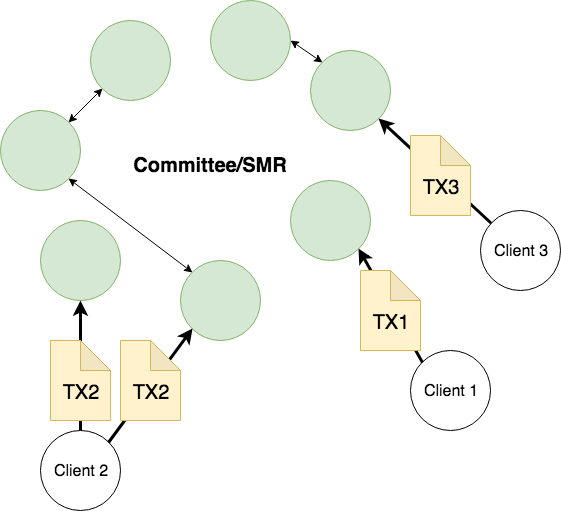
\includegraphics[scale=0.4]{Committee}
\caption{\textbf{Cхематическое изображение алгоритма}}
\label{fig:committee}
\end{figure}

\section{Рассматриваемая модель}
В данном разделе мы опишем модель, в которой работает предложенный алгоритм.

В рамках данной работы мы рассматриваем \textit{инклюзивную} (permissionless) модель, в которой:
\begin{itemize}
\item множество участников алгоритма не фиксировано
\item каждый участник может начать или закончить участие в алгоритме в любое время
\item каждый участник может быть однозначно идентифицирован его публичным ключом и каждый публичный ключ однозначно определяет участника
\item одно устройство может выступать как несколько участников
\end{itemize}

Участники могут быть либо \textit{честными} (honest), либо \textit{неисправными} (faulty).  Честный участник всегда следует предписанному алгоритму, неисправный же может предпринимать действия для нарушения корректной работы алгоритма.
В рамках данной работы мы будем считать, что в комитете находится не более $f$ неисправных участников, и размер комитета $n$ равен $3f+1$.

Что касается неисправных участников, мы считаем, что они могут пытаться скомпрометировать участников коммитета, пытаться подделывать их криптографические зашифрованные данные, взламывать устройство участника, и так далее. Однако, в рамках рассматриваемой модели, данные попытки занимают значительное время, что было формализовано в работе\cite{hybrid-consensus}, и носит название \textit{delayed adaptive adversary}.

Что касается модели сети, участиники сети соединены в пиринговую сеть (peer-to-peer), 
то есть кадждый участник поддерживает соединения с некоторыми другими участниками и обменивается с ними сообщениями. Будем считать, что любой участник может установить с любым другим участником соединение, по которому они могут обмениваться сообщениями. В следующих разделах мы разберем архитектуру сети более подробно.

В рамках данной модели сети будем считать, что отправленное сообщение может быть доставлено не более чем за время $\Delta$, которое является верхней границей на время доставки и известно заранее.
Обозначим $\delta$ как действительное время доставки сообщения от одного участника другому. 
Если время доставки превышает $\Delta$, считаем что участник неисправен, 
то есть $\delta \le \Delta$ для всех честных участников. 
Данная модель сети была формализована в статье Dwork \cite{Dwork:1988:CPP:42282.42283} и называется \textit{частично синхронная}(partially synchronous).

\section{Инклюзивный алгоритм SMR}
В данном разделе мы рассмотрим предложенный алгоритм, 
который является усовершенствованием алгоритма PBFT\cite{pbft} для решения задачи SMR в инклююзивной модели.
 
Так как состав комитета может меняться с течением времени, введем понятие \textit{конфигурация}, обозначающее состав комитета. Пронумеруем конфигурации, таким образом состав комитета ~--- это функция от его номера $c$, которую мы будем обозначать как $C(c)$. 
 
Один из участников в конфигурации является \textit{лидером}, который управляет алгоритмом SMR. 
Остальные участники конфигурации являются \textit{последователями}, которые проверяют и подтверждают действия лидера. Все честные последователи знают, какой участник является лидером.

Лидер в конфигурации может меняться с течением времени, при этом конфигурация может оставаться неизменной. Пронумеруем лидеров в пределах одной конфигурации, обозначив индекс лидера как $v$. Таким образом, лидер ~--- это функция от двух параметров $c$ и $v$: $L(c, v)$.

\subsection{Устойчивое состояние} \label{steady-state}
В данном разделе будет показано, как участники комитета приходят к консенсусу при неизменных $c$ и $v$. Данное состояние постоянности $c$ и $v$ называется \textit{устойчивым состоянием} (steady state).

Прежде всего, введем понятие \textit{лога примененных изменений} ~--- это индексируемый с нуля список, где нулевой элемент в списке ~--- первое примененное изменение, первый элемент ~--- следующее, и так далее. У каждого участника комитета имеется своя копия лога изменений, обозначим ее как $Log_C$, которые были применены к его локальной копии хранилища. \textit{Текущим слотом} будем называть $s$ равную длине $Log_C$. 
В ходе алгоритма, участники сообщения пытаются \textit{заполнить} текущий слот одинаковым сообщением, перейдя к следующему слоту.

Помимо лога и текущего слота каждый участник коммитета хранит следующие данные:
\begin{itemize}
\item номер текущей конфигурации $c$ и номер лидера $v$
\item список публичных ключей всех участников конфигурации с номером $c$ 
\item собственный секретный ключ
\item состояние, которое может обновляться инкрементально
\end{itemize}

Прежде чем перейти к описанию, введем следующее обозначение:
\[ \langle tag, a_1, a_2, ... a_n \rangle_X \] будем обозначать сообщение с тегом $tag$ и полями $a_1$, $a_2$..., $a_n$, подписанное секретным ключом участника $X$. Тег в данном случае ~--- это некоторая строка, которая отличает различные типы сообщений и делает невозможным переиспользование одного сообщения в качестве другого с точно такими же полями.

Теперь опишем как новое изменение попадает в лог участника комитета.

Пусть комитет находится в конфигурации с номером $c$ и лидером с номером $v$. 
Пусть лидер $L$ ($L = L(c, v)$) честный и хочет внести изменение $d$ в логи всех участников комитета. Алгоритм происходит в три раунда.

\textbf{Раунд 1. Предложение}. Лидер отправляет всем участникам конфигурации сообщение 
\[ \langle Propose, c, v, s, d \rangle_L \]

1.1 Каждый честный последователь $F$, получив сообщение, проверяет следующее:
\begin{itemize}
\item $c$, $v$ и $s$ из сообщения равны локальным значениям
\item подпись сообщения корректна и соответствует публичному ключу $L$
\item $proposed_{c, v, s}$ еще не занято другим $\hat d$
\item валидно ли изменение $d$ и возможно ли применить его к состоянию
\end{itemize}

Если все вышеперечисленные проверки выполнились, $F$ присваивает $proposed_{c, v, s} := d$, в противном случае, $F$ игнорирует присланное сообщение. 
\vspace{10pt}

\textbf{Раунд 2. Подготовка}. Каждый честный последователь $F$, для которого выполнились все предыдущие проверки, отправляет лидеру $L$ сообщение 
\[ \langle Prepare, c, v, s, d \rangle_F \]

2.1 Лидер $L$, получив Prepare-сообщение, проверяет, что
\begin{itemize}
\item $c$, $v$ и $s$ из сообщения равны локальным значениям
\item подпись сообщения корректна и соответствует публичному ключу $F$
\item $d$ соответствует сообщению $Propose$ для $s$, отправленному им в предыдущем раунде
\end{itemize}
Если какая-то из проверок не выполнилась, лидер игнорирует присланное сообщение. 

2.2 Лидер дожидается $2f+1$ сообщений $Prepare$ (включая свое собственное) с одинаковыми значением $c$, $v$, $s$ и $d$ и формирует \textit{сертификат согласия} (Acceptance certificate), обозначим его как $\mathcal{P}$. Данный сертификат является гарантией того, что как минимум $2f+1$ участников (среди которых как минимум $f+1$ честных) пришли к согласию, что текущий слот $s$ должен быть заполнен изменением $d$.

Пока для простоты будем считать, что $\mathcal{P}$ ~--- это кортеж
$$(c, v, s, d, \sigma_1, \sigma_2, ..., \sigma_{2f+1})$$
где $Prepare$ ~--- это тег, а $\sigma_i$ ~--- подпись $Prepare$ сообщения $i$-го приславшего участника (включая самого лидера). 
В последующих разделах, формирование сертификата $\mathcal{P}$ будет проанализировано и улучшено.

2.3 После этого лидер отправляет всем последователям  $\mathcal{P}$

2.4 Каждый честный последователь $F$, получив сертификат, проверяет следующее:
\begin{itemize}
\item $c$, $v$, $s$ из сообщения равны локальным значениям
\item $proposed_{c, v, s} = d$
\item все подписи в $\mathcal{P}$ корректны
\end{itemize}
\vspace{10pt}

Если все проверки выполнинились, то участник запоминает данный сертификат в $acceptance_s := \mathcal{P}$.
\vspace{10pt}

\textbf{Раунд 3. Применение}.
Каждый честный последователь $F$, для которого выполнились все предыдущие проверки, отправляет лидеру $L$ сообщение 
\[ \langle Commit, c, v, s, d \rangle_F \]

3.1 Лидер $L$, получив $Commit$-сообщение, проверяет его аналогично шагу 2.1.
Если какая-то из проверок не выполнилась ~--- лидер игнорирует присланное сообщение. 

3.2 Лидер дожидается $2f+1$ сообщений $Commit$ (включая свое собственное) с одинаковыми значением $c$, $v$, $s$ и $d$ и формирует \textit{сертификат применения} (Commit certificate), обозначим его как $\mathcal{C}$.
$$\mathcal{C}=(c, v, s, d, \sigma_1, \sigma_2, ..., \sigma_{2f+1})$$

3.3 После этого лидер отправляет всем последователям  $\mathcal{C}$

3.4 Каждый честный последователь $F$, получив сертификат, проверяет его аналогично шагу 2.4.
Если все проверки выполнились ~--- последователь добавляет изменение $d$ в свой лог и  применяет изменение $d$ к своему локальному состоянию.
\vspace{10pt}

Следует отметить, что лидер следует всем шагам алгоритма действуя и как лидер, и как последователь. За исключением того, что он не отправляет сообщения самому себе.

Будем называть сертификат \textit{корректным}, если все подписи в нем корректны.
Стоит обратить внимание, что вообще говоря два последователя $F_1$ и $F_2$ могут получить разные корректные сертификаты согласия $\mathcal{P}_1$ и $\mathcal{P}_2$ и/или применения $\mathcal{C}_1$ и $\mathcal{C}_2$, однако, это не нарушает корректность алгоритма, при условии что сертификаты корректны.
То есть лидер может дождаться более чем $2f+1$ $Prepare$/$Commit$ сообщения и сформировать каждому последователю корректный сертификат, отличный от других.

Также, если лидер отправляет последователю сертификат для $s$, в то время как последователь уже имеет корректный сертификат для $s$, то последователь игнорирует присланный.

\subsection{Реконфигурация}
В данном разделе будет описано, как комитет переходит в новую конфигурацию, то есть как обновляется состав комитета. Данный шаг называется реконфигурация ~--- то есть изменение конфигурации.

Cхема реконфигурации состоит в том, что \textit{майнеры} ~--- участники сети, которые хотят вступить в комитет, совершают работу по решению некоторого \textit{паззла}. После того как решение найдено, майнер публикует данное решение в комитет, каждый участник комитета проверяет найденное решение, и отвечает майнеру сообщением подтверждением, что решение корректно и участник готов принять его в комитет.
После чего, текущий лидер комитета предлагает изменение, которое добавляет майнера в комитет.

Формально, решение паззла ~--- это некоторое число $\phi$, что:
$$\mathcal{H}(puzzle_c, pk, \phi) \le target$$
где $\mathcal{H}$ ~--- криптографически стойкая хэш-функция, $puzzle_c$ ~--- это некоторая величина, зависящая от $c$, называемая \textit{паззлом}, $pk$ ~--- публичный ключ майнера, $target$ ~--- некоторое число, которое задает сложность вычисления.

Другими словами, майнеры выполняют доказательство выполненной работы (PoW), подобно тому, как это делается в Bitcoin.  Число $target$ выбирается так, чтобы поиск числа $\phi$ примерно занимал некоторое время $D$, намного большее $\Delta$. Скажем, $D$ равное 10 минутам, как и в Bitcoin подойдет.  $target$ также меняется со временем, и зависит от частоты нахождения предыдущих значений $PoW$, более подробно с тем, как выбирается $target$ можно познакомиться в оригинальной статье [ссылка].
Как формируется число $puzzle_c$ будет рассказано далее в этом разделе, на данный момент важно лишь то, что паззл зависит от номера конфигурации. Сосредоточимся более подробно на том, как майнер добавляется в комитет.

Майнера, который нашел число $\phi$, будем называть \textit{кандидатом}.
Прежде всего, каждый участник комитета для конфигурации $c$ хранит множество известных ему кандидатов $Q_c$.
\vspace{10pt}

Итак, после того, как майнер $W$ нашел число $\phi$, он отправляет всем участникам комитета сообщение
 \[ \langle Candidate, c, puzzle_c, pk, \phi \rangle_W \]
 
Участник $M$, получивший данное сообщение, выполняет следующую последовательность шагов:

1.1 Берет эксклюзивную блокировку $B$ на чтение данных. То есть откладывает обработку сообщения от лидера $L(c, v)$ до тех пор, пока блокировка не будет отпущена. 

1.2. Проверяет, что выполняется все из следующего:
\begin{itemize}
\item корректность подписи $W$ 
\item корректность решения пазла, то есть что $\mathcal{H}(puzzle_c, pk, \phi) \le target$
\item $c$ из сообщения равно локальному значению
\end{itemize}

1.3. Засекает таймер $T$ на $5\Delta$ и отправляют кандидату $W$ сообщение:
 \[ \langle Status, c, v, s, pk \rangle_M \]
где $c$, $v$~--- локальные  $c$, $v$, $pk$~--- публичный ключ $W$.
\vspace{10pt}

После того как $W$ получает $2f+1$ корректно подписанных $Status$ сообщений с одинаковыми $(c, v)$, он вычисляет $s^{*}=max(s_1, s_2,..., s_{2f+1})+2$, где $s_i$~--- слоты из $Status$ сообщений.
Далее отправляет всем участникам запрос на подтверждение слота:
 \[ \langle ReserveSlot, c, v, s^{*} \rangle_W \]
 
\noindent Участник $M$, получивший это сообщение, проверяет:
\begin{itemize}
\item корректность подписи W
\item $c$ и $v$ равны локальным значениям
\item $proposed_{c, v, s^{*}}$ еще не заполнено никаким изменением $d'$
\end{itemize} 
После чего отправляет в ответ $W$:
 \[ \langle ConfirmSlot, c, v, s^{*}, pk \rangle_M \]
где $pk$~--- публичный ключ $W$.
\vspace{10pt}

После получения $2f+1$ корректно подписанных $Confirm$, с одинаковыми значениями $c$, $v$ и $s^{*}$,
формирует и отправляет всем участникам комитета \textit{сертификат кандидата} $\mathcal{S}$:

$$\mathcal{S}=(c, v, s^{*}, pk, \sigma_1, \sigma_2,..., \sigma_{2f+1})$$
$\sigma_i$ ~--- подписи $ConfirmSlot$ сообщений.
\vspace{10pt}

Участник $M$, получивший данное сообщение, выполняет шаги : 

2.1. Проверяет подписи $ConfirmSlot$ сообщений $\sigma_i$.

2.2. Добавляет $\mathcal{S}$ в $Q_c$.

2.3. Отправляет данный сертификат всем остальным участникам комитета.

2.4. Снимает блокировку на ресурсы $B$.

Если кандидат не успевает прислать сертификат $\mathcal{S}$ до истечения таймера $T$, блокировка $B$ снимается.

Данная процедура во-первых гарантирует, что либо все честные участники, либо ни одного (в зависимости от честности действий кандидата) узнают о новом кандидате, а во-вторых что как минимум $f+1$ честных участников придут к консенсусу о $s^{*}$.

После того, как все честные участники, в том числе и лидер $L(c, v)$, узнали о кандидатах, претендующих на добавление в комитет, участники ожидают от лидера, что в скором времени лидер предложит изменение, которое изменит конфигурацию комитета. А именно, каждый раз, когда участник получает $Propose$ сообщение, помимо проверок описанных в  разделе \ref{leader-change}, он проверяет, что данное сообщение $Propose$ содержит тех, и только тех кандидатов из $Q_c$, для которых выполяется $s^{*} = s$, где $s$~--- слот из $Propose$ сообщения. Если же это условие не выполняется, участник игнорирует данное $Propose$ сообщение.

Изменение реконфигурации $d_{rec}$ формально описывается следующим образом:
$$d_{rec}=(c, puzzle_c, (pk_1, \phi_1, \sigma_1), (pk_2, \phi_2, \sigma_2),...,(pk_k, \phi_k, \sigma_k))$$
где $k$~--- количество кандидатов, $\sigma_i$~--- подпись $Candidate$ сообщения.

Как только $d_{rec}$ будет применено и попадет в лог применений, необходимо произвести реконфигурацию.
Реконфигурация задается функцией $\Phi$ из изменения реконфигурации в список кандидатов. Данная функция определяет каких кандидатов и в каком порядке необходимо добавить в комитет, следовательно, столько же самых давних участников должны покинуть его. Для простоты рассмотрим $\Phi$, которая возвращает кандидата, у которого решение пазла является наименьшим, то есть $\mathcal{H}(puzzle_c, pk, \phi)$ наименьше, а при равенстве, выберем c наименьшим $pk$.

Итак, после того как участник $M$ получил сертификат применения $d_{rec}$, он выполняет следующие шаги:

3.1. Отправляет его всем остальным участникам

3.2. Проверяет, является ли он самым давним участником, покидает комитет и перестает выполнять дальнейшие шаги. 

В противном случае выполняет последующие шаги алгоритма:

3.3. Вызывает процедуру актуализации лога применений (которая будет описана в разделе \ref{act_log})

3.4. Добавляет $d_{rec}$ в лог применений

3.5. Вычисляет $pk=\Phi(d_{rec})$

3.6. Добавляет кандидата $pk$ в список участников комитета и убирает самого старого из списка

3.7. Заводит $Q_{c+1} := \{\}$

3.8. Отправляет вновь добавленному кандидату сообщение $\langle Welcome, c+1, \mathcal{C} \rangle_M$, где $\mathcal{C}$~--- сертификат применения $d_{rec}$.

3.9. Присваивает $L(c+1, 0):=pk$.

3.10. Вычисляет $puzzle_{c+1}=$ \textbf{TODO}.

3.11. Увеличивает $c$ на один и обнуляет $v$

3.12. Запускает процедуру актуализации лога применений для сертификата $d_{rec}$, которая описана в разделе \ref{act_log}.

После того, как кандидат $W$ получит $f+1$ корректное $Welcome$ сообщение, он начинает действовать как лидер комитета. В данный момент реконфигурация считается проведенной успешно и комитет переходит в новое устойчивое состояние.

\subsection{Смена лидера} \label{leader-change}
В данном разделе будет описано, как участники комитета переходят к лидеру с номером $v+1$, если текущий лидер препятствует прогрессу системы. Прежде всего опишем, как последователь обнаруживает \textit{отстутствие прогресса}.

Будем считать, что лидер производит изменения довольно часто. В следующих разделах будет пояснено, почему данное предположение корректно.

После очередного применения некоторого изменения $d$ или смены лидера последователь $M$ запускает таймер на время $6\Delta$ ~--- за это время честный лидер должен успеть провести 3 раунда описанных выше, и последователь должен получить следующее изменение.
Данная величина получена из следующих соображений, что последователи обмениваются с лидером пятью сообщениями, и так как мы считаем, что в рамках данной модели сообщение отправленное честным участником не должно идти дольше времени $\Delta$, данная процедура не должна занять больше $5\Delta$. Делая поправку на погрешность, а также учитывая то, что проверка сообщений также занимает некоторое время, добавляем к этом времени еще $\Delta$.

После того, как последователь $M$ обнаружил отсутствие прогресса, то есть состояние, при котором текущий лидер не предложил новое измнение за время $6\Delta$, последователь переходит в \textit{состояние смены лидера}.
Результат выхода из этого состояния будет следующее устойчивое состояние с новыми $c$ и $v$.
Цель описанного далее процесса~--- сформировать сертификат \textit{устойчивого состояния}:
$$\mathcal{W}=(c, v', s^{*}, \mathcal{C}^{*}, \mathcal{P}^{*}, Q^{*}, \sigma_{L(c, v')}, \varkappa_1, \varkappa_2,..., \varkappa_{2f+1})$$

Данный сертификат содержит значения $c, v', s$, на которых участники согласовываются, переходя в новое устойчивое состояние, а также о последних имеющихся у участников сертификатах согласия и множествах кандидатов.

Итак, после того, как участник $M$ перешел в состояние смены лидера, он проделывает следующее:

1.1. Перестает принимать сообщения с тегом отличным от $LeaderChange$ и $NewLeader$

1.2. Отправляет сообщение новому лидеру $L(c, v+1)$:
\[ \langle LeaderChange, c, v+1,  \hat{\mathcal{C}}, \hat{\mathcal{P}}, Q_c \rangle_M \]
где $\hat{\mathcal{C}}$ и $\hat{\mathcal{P}}$~--- последнний сертификат применения и согласия, полученный $M$, $Q_c$~--- известные $M$ кандидаты.

1.3. Засекает таймер на $6\Delta$.

1.4. Если таймер истек, $M$ не перешел в новое устойчивое состояние, то он повторяет шаги 2 и 3 для следующего лидера $v+2$. Данный шаг будет повторяться до тех пор, пока $M$ не окажется в устойчивом состоянии.
\vspace{10pt}

После того, как новый лидер $L(c, v')$ получит $2f+1$ корректно подписанных сообщений $LeaderChange$ с одинаковыми $c$ и $v'$  (включая свое) далее формирует отправляет всем участникам:
\[ \langle Election, c, v', \hat{\mathcal{C}}_1,...,\hat{\mathcal{C}}_{2f+1}, \hat{\mathcal{P}}_1,...,\hat{\mathcal{P}}_{2f+1}, Q_1,..., Q_{2f+1}, \sigma_1,..., \sigma_{2f+1}\rangle_{L(c, v')} \]

Получив данное сообщение участник $M$:
\begin{itemize}
\item подпись $Election$ корректна
\item значение $c$ из сертификата совпадает с локальным
\item $v'$ строго больше локального $v$
\item корректность всех $\hat{\mathcal{P}}_i$ и $\hat{\mathcal{C}}_i$
\item корректность всех подписей $\sigma_i$
\end{itemize}
Если хотя бы одна из проверок не выполнилась, $M$ игнорирует сообщение, иначе выполняет следующее:

2.1. Находит сертификат $\mathcal{C}^{*}$, в котором значение слота наибольшее и равно $s^{*}$, аналогично $\mathcal{P}^{*}$ вместе с  $s_P^{*}$, причем если существует несколько сертификатов согласия с $s_P^{*}$, участник выбирает с наибольшим значением $(c, v)$, а также вычисляет $Q^{*}=\bigcup\limits_{i=1}^{2f+1} Q_i$.

2.2. Отправляет лидеру в ответ
\[ \langle Vote, c, v', s^{*}, \mathcal{C}^{*}, \mathcal{P}^{*}, Q^{*}, \sigma_{L(c, v')} \rangle_M \]
где $\sigma_{L(c, v')}$~--- подпись сообщения $Election$.
\vspace{10pt}

Получив $2f+1$ $Vote$ сообщений с одинаковыми $c, v', \mathcal{C}^{*}, \mathcal{P}^{*}, Q^{*}, \sigma_{L(c, v')}$, новый лидер $L(c, v')$ формирует и отправляет сертификат \textit{устойчивого состояния}:
$$\mathcal{W}=(c, v', s^{*}, \mathcal{C}^{*}, \mathcal{P}^{*}, Q^{*}, \sigma_{L(c, v')}, \varkappa_1, \varkappa_2,..., \varkappa_{2f+1})$$
$\varkappa_i$ ~--- это подпись $Vote$ сообщения $i$-го приславшего участника.

После того как участник $M$ получил сертификат, он проверяет следующее:
\begin{itemize}
\item значение $c$ из сертификата совпадает с локальным
\item $v'$ строго больше локального $v$
\item слот $s^{*}$ соответствует $\mathcal{C}^{*}$
\item корректность всех $\mathcal{C}^{*}$ и $\mathcal{P}^{*}$
\item корректность всех подписей $\varkappa_i$
\end{itemize}
Если хотя бы одна из проверок не выполнилась, $M$ игнорирует сообщение. В противном случае:

3.1. Отправляет всем участникам $\mathcal{W}$

3.2. Проводит процедуру актуализации лога применений с $\mathcal{C}^{*}$

3.3. Обновляет $Q_c := Q^{*}$.

3.4. Обновляет $v := v'$ и тем самым \textit{принимает} нового лидера.

3.5. Обновляет $acceptance_{s_P^{*}} := \hat{\mathcal{P}}^{*}$

6. В случае если $s_P^{*}=s^{*}+1$, отправляет
\[ \langle Commit, c, v', s_P^{*}, d^{*} \rangle_F \]
где $d^{*}$ изменение из $\mathcal{P}^{*}$ и дожидается сертификата применения от $L(c, v')$, после чего участник переходит в новое устойчивое состояние, присваивая $leaderChange := False$, иначе по истечению таймера переходит к смене лидера.

3.7. Если условие в шаге 6 не выполнилось, то есть $s^{*}=s_P^{*}$, переходит в новое устойчивое состояние после шага 6, присваивая $leaderChange := False$.

Стоит обратить внимание, что участник $M$ может уже иметь сертификат применения для $s_P^{*}$, $d^{*}$, однако в случае выполнения  шага 6, он все равно отправляет $Commit$ сообщение.

Процедура смены лидера несет две цели: достигнуть консенсуса о новом лидере, а также актуализировать логи всех честных участников, устраняя отставание, которое мог создать предыдущий лидер.

В следующей главе будет доказано, что либо $s_P^{*}=s^{*}$, либо $s_P^{*}=s^{*}+1$, то есть либо сертификат согласия соответствует сертификату применения, либо сертификат согласия соответствует предложенному предыдущим лидером изменению.

\subsection{Процедура актуализации лога применений} \label{act_log}
Процедура актуализации лога применений необходима для устранения отставания участника комитета.
Она принимает на вход текущий слот участника $s$ и сертификат согласия или применения $\mathcal{D}$, имеющийся у участника.

Обозначим $s$ текущий слот участника комитета $M$, а $s_k$ номер слота из сертификата. Если $s \le s_k-1$, тогда $M$ отправляет любым $f+1$ участникам из сертификата 
\[ \langle RequestCommits, s, s_k-1 \rangle_M \]
тем самым запрашивая изменения соответствующие слотам $s, s+1,..., s_k-1$

Участник $M'$, получивший данное сообщение и имеющий сертификаты применения для соответствующих слотов, отправляет их в ответ
\[ \langle ReponseCommits, \mathcal{C}_s, \mathcal{C}_{s+1},...,\mathcal{C}_{s_k-1} \rangle_{M'} \]

Получив их $M$ проверяет корректность каждого из них и применяет изменения к состоянию, добавляя их после этого в лог применений. Таким образом процедура гарантирует, что в лог применений будет заполнен по слот $s_k-1$ включительно.

\subsection{Стартовый запуск}

\section{Взаимодействие комитета с клиентами}

\section{Микроблоки}

\section{Уменьшение размера сертификата}


